\section{Projektplanung}

\subsection{Entwicklungsprozess}

Um das Projekt realisieren zu können, musste sich für einen geeigneten Entwicklungsprozess entschieden werden. Dieser gibt die Vorgehensweise vor, welche der Umsetzung zu Grunde liegt. Für dieses Projekt wurde vom Autor das Wasserfallmodell gewählt. Dabei wird die Umsetzung auf fünf Phasen aufgeteilt (siehe \autoref{fig:wasserfallmodell}): Ermittlung der Anforderungen,  Erstellung eines Entwurfs, Implementierung, Überprüfung und Wartung der erstellten Software. Dieses Modell bietet sich für diese Arbeit an, da die Anforderungen an den Editor klar definiert sind und sich während der Umsetzungsphase nicht ändern.

\begin{figure}[H]
	\centering
	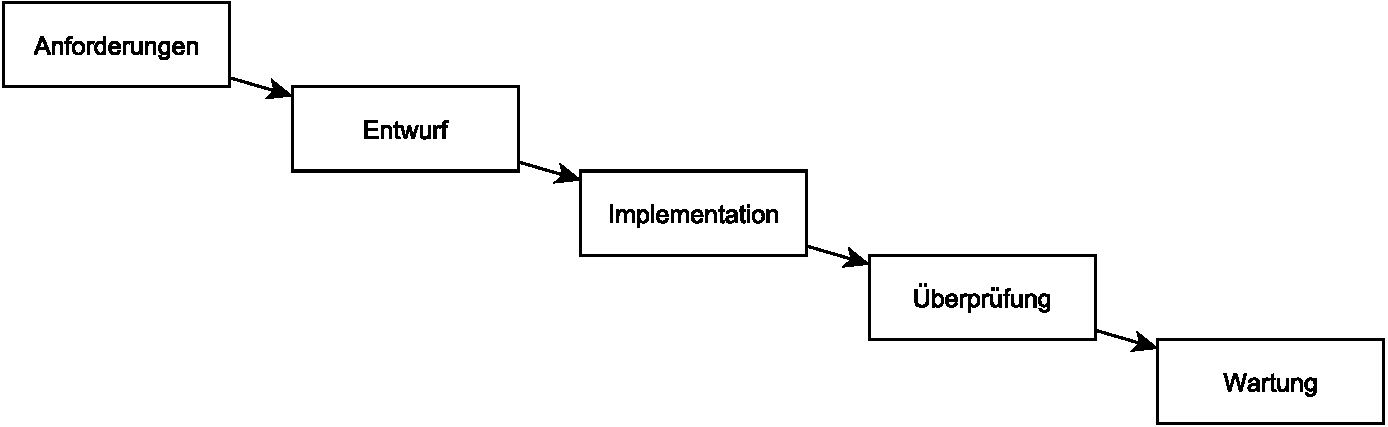
\includegraphics[height=110px]{../graphic/diagrams/SD_Wasserfallmodell/Wasserfallmodell}
	\caption{Wasserfallmodell}
	\label{fig:wasserfallmodell}
\end{figure}

\subsection{Projektphasen}
\label{Projektphasen}

Zur Realisierung des Abschlussprojekts standen insgesamt 70 Stunden zur Verfügung. Diese Zeit wurde vor Projektbeginn auf verschiedene Phasen verteilt, die während der Durchführung durchlaufen werden. Die Zeitplanung lässt sich aus \autoref{fig:grobeZeit} entnehmen.

\begin{figure}[H] 
	\begin{center}
		\begin{tabularx}{0.90\textwidth}{X|P{50px}|P{50px}}
			\hline \rowcolor{ADITO_RED} \textcolor{white}{\textbf{Vorgang}} & \textcolor{white}{\textbf{Geplante Zeit in h}} 	\\
			\hline
			1. Analysephase													& 3 	\\ 
			
			2. Entwurfsphase						 						& 15 	\\
			
			3. Implementierungsphase										& 40	\\
			
			4. Testphase													& 2 	\\
			5. Dokumentationserstellung										& 10 	\\ 
			\hline 
			& 70 \\
		\end{tabularx}
	\end{center}
	\caption{Grobe Zeitplanung} 
	\label{fig:grobeZeit}
\end{figure}

\subsection{Ressourcenplanung}

Im Zuge der Ressourcenplanung wurde eine Übersicht (siehe Anhang \ref{ressources}) erstellt. Diese enthält sämtliche Ressourcen, welche innerhalb der Durchführung des Projekts eingesetzt wurden. Dabei handelt es sich sowohl um Hard- und Softwareressourcen als auch um Personal. Zur Minimierung der Projektkosten wurde bevorzugt kostenfreie Software verwendet. War dies nicht möglich, so wurde Software eingesetzt, für welche die ADITO Software GmbH bereits Lizenzen besaß.



\newpage